% ----------------------------------------------------------
\chapter{Fundamentação Teórica}\label{cap:fundamentacaoTeorica}
% ----------------------------------------------------------
Explicar brevemente o que será tratado como fundamentação teórica para o entendimento do contexto em que o modelo de aprendizagem de máquina será aplicado.

\section{A importância da cadeia de suprimentos}

Embora a globalização do mundo tenha tomado força no início do século XXI, intensificando a importação e exportação de matéria prima, commodities e produtos entre os países, a logística e o gerenciamento da cadeia de suprimentos são conceitos que impactam o desenvolvimento da humanidade há séculos. Desde a construção de pirâmides, até os esforços humanitários para a dimiuição da fome em países africanos se fundamentam no fluxo eficiente de materiais e insumos para que estes objetivos sejam alcançados.

Além disso, nas últimas guerras travadas pela humanidade, a capacidade logística foi um fator determinante para os países que saíram vitoriosos na história. Seja na estratégia para levar armamento ao território hostil, como também nos ataques a navios e comboios com comida e medicamentos para os soldados em combate, assegurar o planejamento e execução do transporte de materiais, e comprometer fluxo logístico do inimigo podia significar um passo adiante para a vitória na guerra. 

O Imperador Alexandre, o Grande, disse uma vez: "Meus especialistas em logística são muito sérios… pois sabem que, se minha campanha falhar, serão os primeiros que matarei". A afirmação mostra o quão importante a cadeia de suprimentos era para o império naquela época. Trazendo essa importância para a ótica dos dias atuais, basta olhar todos os móveis, itens de decoração, utensílios e ferramentas, seja do ambiente doméstico ou do trabalho, que se nota a necessidade dessa cadeia para tudo estar aonde está.

Mais do que um processo que está por trás da produção e envio de mercadorias ao redor do globo, a boa governança de uma cadeia de suprimentos constitui uma infraestrutura vital para o funcionamento e o desenvolvimento sustentável da sociedade.

\section{A gestão global da cadeia de suprimentos e seus desafios}

Segundo a empresa de tecnologia Totvs, "A cadeia de suprimentos (do inglês, \textit{supply chain}) é um sistema que envolve pessoas, processos e tecnologias focados em um objetivo: na melhor entrega possível de valor a um cliente, envolvendo todas as etapas de fabricação e entrega de produtos". 

Vale ressaltar a diferença entre a gestão logística e a gestão da cadeia de suprimentos (do inglês, \textit{Supply Chain management}, SCM), dado que a primeira está contida na segunda. Ao realizar toda essa gestão, estão incluídas todas as atividades que transformam matérias-primas em  produtos acabados para uso dos clientes, como o sourcing, design, produção, armazenamento, expedição e distribuição, ilustrado na Figura \ref{fig:Fig_1}

\begin{figure}[htb]
	\caption{\label{fig:Fig_1}Fluxo do SCM.}
	\begin{center}
		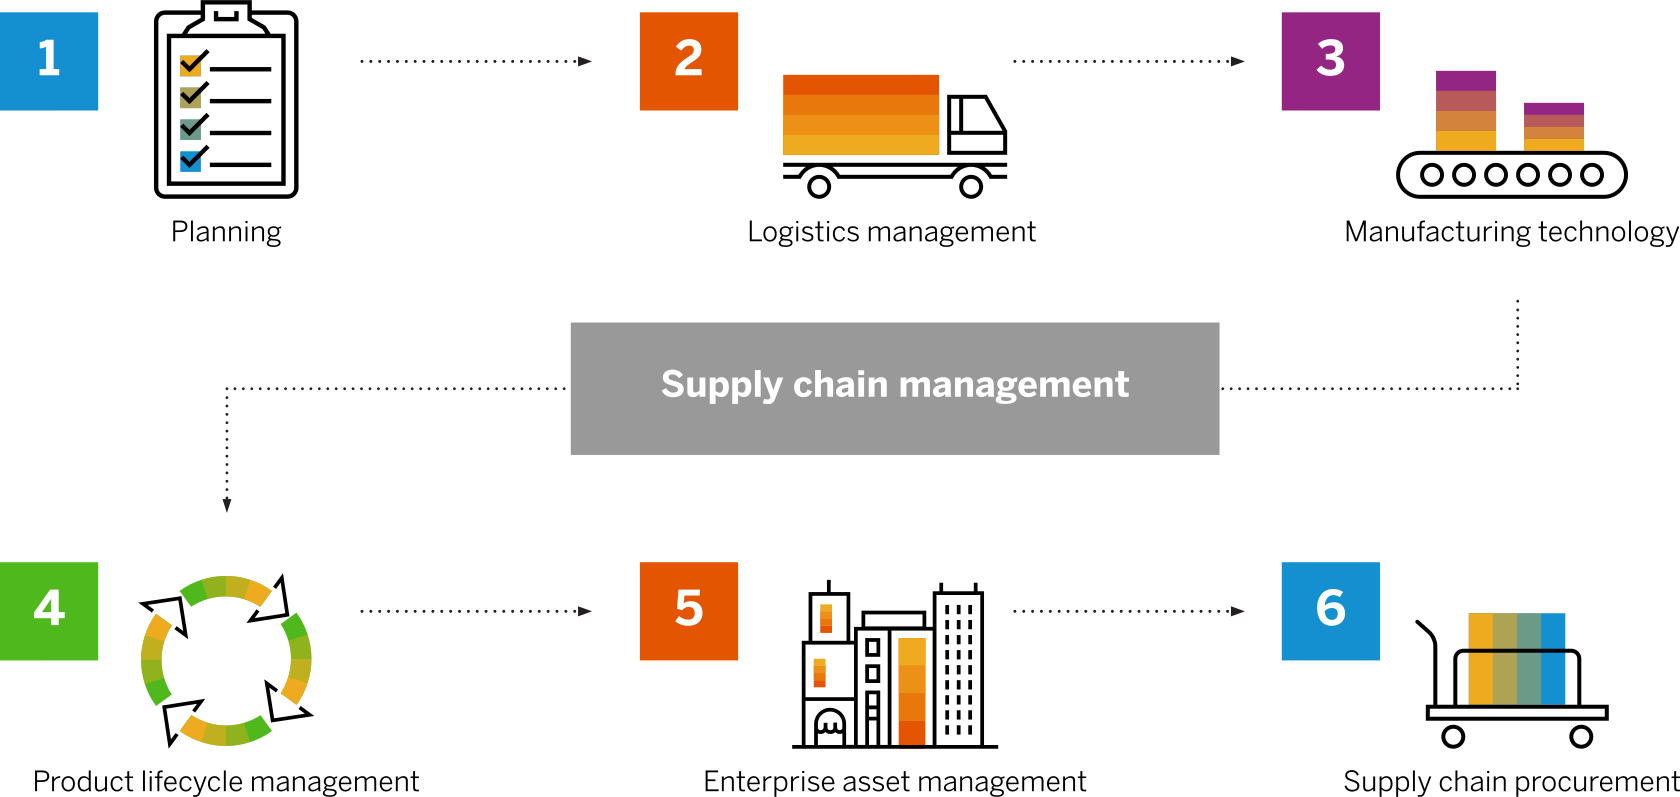
\includegraphics[scale=0.2]{figuras/what-is-supply-chain-management-graphic.png}
	\end{center}
	\fonte{Referência SAP}
\end{figure}

O gerenciamento da cadeia de suprimentos é essencial para a eficiência operacional e manutenção da competitividade de uma empresa no seu ramo de atuação. Um bom gerenciamento garante níveis de inventário que atendam às necessidades de produção, sem, ao mesmo tempo, gerar excessos que resultem em custos desnecessários ou em faltas de materiais que comprometam a capacidade de entrega no prazo. Tudo isso envolve um equilíbrio tênue entre a demanda prevista e a disponibilidade de suprimentos. 

Em condições normais de mercado, esse gerenciamento já é complexo, exigindo uma análise constante de dados de vendas, previsões de demanda e ajustes rápidos para evitar rupturas de estoque ou excessos. Sob condições atípicas, como as vivenciadas durante a pandemia, esse desafio se multiplica. A incerteza dos mercados, as restrições de fornecimento e as mudanças de comportamento do consumidor criam um cenário de alta volatilidade, exigindo um gerenciamento de estoque ainda mais dinâmico e ágil.

A crise dos semicondutores de 2021-2022 evidenciou as fragilidades das cadeias globais desse produto. Enquanto a demanda por chips disparou nesse período, a produção concentrada em poucos países, que ainda se recuperavam dos efeitos da pandemia, gerou escassez em diversas áreas da economia. O setor automotivo teve uma queda da produção de 15 milhões de veículos, e até mesmo o aprimoramento do acelerador de partículas LHC sofreu com adiamentos devido a falta de chips para o projeto. 

Através desses eventos, as empresas e nações evidenciaram a necessidade urgente da modernização dos processos de SCM, sendo mais flexíveis e resilientes a mudanças porém sem perder a estabilidade. Hoje, as melhores companhias analisam as operações dentro da área e suas tecnologias de execução, levantando questionamentos do que fazer para tornar os negócios mais eficientes, lucrativos e prontos para o futuro.

\section{Princípio de Pareto}

O Princípio de Pareto surgiu inicialmente no final do século XIX, quando o economista e sociólogo Vilfredo Pareto (1848-1923) notou que 80\% da riqueza de seu país (Itália) vinha de 20\% da população. Intrigado com a descoberta, Pareto aplicou a mesma lei a outros países como Rússia, França e Suíça, chegando ao mesmo resultado.

Mesmo após validar sua teoria em outros países, o Princípio de Pareto só foi reconhecido nos anos 40, pelo engenheiro americano Joseph Juran (1094-2008) ao aplicar a teoria na área da qualidade, e comprová-la em outras situações além das constatadas por Pareto.

De acordo com Antoine Delers, "o modelo provém da observação de que 20\% das causas são responsáveis por 80\% dos efeitos". 

Criar ligação do princípio de Pareto com as Classificações ABC-FMR

\subsection{Classificação ABC}

A classificação ABC é um método de categorização de materiais com base na importância relativa desses itens para uma organização. Os itens são classificados em três categorias principais - A, B e C - de acordo com seu valor ou impacto no desempenho geral da empresa.

\begin{itemize}
	\item Itens da Categoria A: agrega os itens de maior valor ou impacto, geralmente representando uma porcentagem significativa do valor total dos estoques ou das vendas. Esses itens são considerados críticos para o sucesso da empresa e requerem uma gestão mais rigorosa e atenção especial.
	\item Itens da Categoria B: classifica itens de valor moderado, que representam uma parte intermediária do valor total dos estoques ou das vendas. Embora não sejam tão críticos quanto os itens da Categoria A, os materiais dessa categoria ainda requerem um nível razoável de controle e monitoramento.
	\item Itens da Categoria C: itens de menor valor ou impacto, geralmente representando uma pequena parte do valor total dos estoques ou das vendas. Esses itens são considerados menos críticos e podem exigir menos atenção em comparação com os itens das categorias A e B.
\end{itemize}

Através da classificação ABC, a empresa dispõe de uma análise mais objetiva na gestão de estoques, compras e planejamento de produção, a fim de priorizar a alocação de recursos e esforços com base na importância relativa dos itens.

\subsection{Classificação FMR}

A classificação FMR é um método complementar à classificação ABC, utilizado para categorizar itens com base na frequência de demanda ou movimentação. A categorização dos materiais com base nessa classificação ajuda a determinar a estratégia de gestão de estoque mais adequada para cada item, considerando a sua movimentação no sistema.

\begin{itemize}
	\item Itens da categoria F (\textit{Fast Mover}): Itens com alta frequência de demanda ou movimentação. São produtos que têm uma alta rotatividade e são frequentemente solicitados pelos clientes. Esses itens geralmente requerem um estoque mais robusto para garantir disponibilidade imediata.
	\item Itens da categoria  M (\textit{Medium Mover}): Itens com uma frequência de demanda moderada. Embora não sejam tão solicitados quanto os itens da categoria F, esses produtos ainda têm uma demanda significativa e precisam ser gerenciados com atenção para evitar rupturas de estoque.
	\item Itens da categoria R (\textit{Rare Mover}): Itens com baixa frequência de demanda ou movimentação. São produtos que têm uma demanda esporádica ou sazonal, e geralmente não são solicitados com frequência. Esses itens podem não precisar de um estoque tão grande e podem ser gerenciados de forma mais flexível.
\end{itemize}

Além de classificar a frequência de demanda de um material, a classificação FMR também é útil para determinar se um item deve ser mantido em estoque (\textit{Make to Stock} - MTS) ou produzido sob demanda (\textit{Make to Order} - MTO). Desse modo, itens classificados como F podem ser mais adequados para a estratégia MTS, enquanto itens da categoria R são tratados para a estratégia MTO.

É a parte principal e mais extensa do trabalho. Deve apresentar a fundamentação teórica, a metodologia, os resultados e a discussão. Divide-se em seções e subseções conforme a NBR 6024 \cite{NBR6024:2012}.

Quanto à sua estrutura e projeto gráfico, segue as recomendações da norma para preparação de trabalhos acadêmicos, a NBR 14724, de 2011 \cite{NBR14724:2011}.

\begin{figure}[htb]
	\caption{\label{fig:Fig_2}Elementos do trabalho acadêmico.}
	\begin{center}
		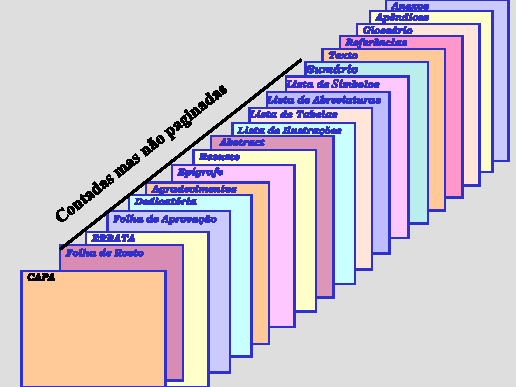
\includegraphics{figuras/imagem.pdf}
	\end{center}
	\fonte{Universidade Federal do Paraná (1996).}
\end{figure}

\subsection{Formatação do texto}

No que diz respeito à estrutura do trabalho, recomenda-se que:
\begin{alineas}
	\item o texto deve ser justificado, digitado em cor preta, podendo utilizar outras cores somente para as ilustrações;
	\item utilizar papel branco ou reciclado para impressão;
	\item \textbf{se o trabalho for impresso}, os elementos pré-textuais devem iniciar no anverso da folha, com exceção da ficha catalográfica ou ficha de identificação da obra;
	\item \textbf{se o trabalho for impresso}, os elementos textuais e pós-textuais devem ser digitados no anverso e verso das folhas;
	\item as seções primárias devem começar sempre em páginas ímpares, quando o trabalho for impresso e
	\item deixar um espaço entre o título da seção/subseção e o texto e entre o texto e o título da subseção.
\end{alineas}

No \autoref{qua:Quadro_1} estão as especificações para a formatação do texto.

\begin{quadro}[htb]
	\centering
	\caption{\label{qua:Quadro_1}Formatação do texto.}	
	\begin{tabular}{|l|p{11cm}|}
		\hline
		\textbf{Formato do papel} & A4.\\ \hline
		\textbf{Impressão}        & A norma recomenda que \textbf{caso seja necessário imprimir}, deve-se utilizar a frente e o verso da página.\\ \hline
		\textbf{Margens}          & Superior: 3, Inferior: 2, Interna: 3 e Externa: 2. Usar margens espelhadas quando o  trabalho for impresso.\\ \hline
		\textbf{Paginação}        & As páginas dos elementos pré-textuais devem ser contadas, mas não numeradas. Para trabalhos digitados somente no anverso, a numeração das páginas deve constar no canto superior direito da página, a 2 cm da borda, figurando a partir da primeira folha da  parte textual. Para trabalhos digitados no anverso e no verso, a numeração deve constar no canto superior direito, no anverso, e no canto superior esquerdo no verso.\\ \hline
		\textbf{Espaçamento}      & O texto deve ser redigido com espaçamento entre linhas 1,5, excetuando-se as citações de mais de três linhas, notas de rodapé, referências, legendas das ilustrações e das tabelas, natureza (tipo do trabalho, objetivo, nome da instituição a que é submetido e área de concentração), que devem ser digitados em espaço simples, com fonte menor. As referências devem ser separadas entre si por um espaço simples em branco.\\ \hline
		\textbf{Paginação}        & A contagem inicia na folha de rosto, mas se \textbf{insere o número da página na introdução} até o final do trabalho.\\ \hline
		\textbf{Fontes sugeridas} & Arial ou Times New Roman.\\ \hline
		\textbf{Tamanho da fonte} & \textbf{Fonte tamanho 12 para o texto}, incluindo os títulos das seções e subseções. As citações com mais de três linhas, notas de rodapé, paginação, dados internacionais de catalogação, legendas e fontes das ilustrações e das tabelas devem ser de tamanho menor. Adotamos, neste \textit{template} \textbf{fonte tamanho 10}.\\ \hline
		\textbf{Nota de rodapé}   & Devem ser digitadas dentro da margem, ficando separadas por um espaço simples por entre as linhas e por filete de 5 cm a partir da margem esquerda. A partir da segunda linha, devem ser alinhadas embaixo da primeira letra da primeira palavra da primeira linha.\\ \hline
	\end{tabular}
	\fonte{\textcite{NBR14724:2011}.}
\end{quadro}


\subsubsection{As ilustrações}

Independentemente do tipo de ilustração (quadro, desenho, figura, fotografia, mapa, entre outros), a sua identificação aparece na parte superior, precedida da palavra designativa. 

\begin{citacao}
	Após a ilustração, na parte inferior, indicar a fonte consultada (elemento obrigatório, mesmo que seja produção do próprio autor), legenda, notas e outras informações necessárias à sua compreensão (se houver). A ilustração deve ser citada no texto e inserida o mais próximo possível do texto a que se refere. \cite[p. 11]{NBR14724:2011}.
\end{citacao}

\subsubsection{Equações e fórmulas}

As equações e fórmulas devem ser destacadas no texto para facilitar a leitura.  Para numerá-las, usar algarismos arábicos entre parênteses e alinhados à direita. Pode-se adotar uma entrelinha maior do que a usada no texto \cite{NBR14724:2011}.

Por exemplo, a circunferência e a área de um círculo com raio $r$ são dados, respectivamente, por
\begin{equation}\label{eq:Eq_1}
\gls{C} = 2 \gls{pi} \gls{r}    %note que o comando \gls{} usa a definição da lista de símbolos. Se não houver lista de símbolos, a equação deve ser digitada normalmente, ou seja, C = 2 \pi r
\end{equation}
e
\begin{equation}\label{eq:Eq_2}
\gls{A} = \gls{pi} \gls{r}^2.
\end{equation}
É importante observar que a \autoref{eq:Eq_1} e a \autoref{eq:Eq_2} fazem parte da frase (note a letra ``e'' entre as equações e o ponto final após a \autoref{eq:Eq_2}). 

\subsubsubsection{Exemplo tabela}

De acordo com \textcite{ibge1993}, tabela é uma forma não discursiva de apresentar informações em que os números representam a informação central. Ver \autoref{tab:Tab_1}.

\begin{table}[htb]
	\ABNTEXfontereduzida
	\caption{\label{tab:Tab_1}Médias concentrações urbanas 2010-2011.}
	\begin{tabular}{@{}p{3.0cm}p{1.5cm}p{2cm}p{2.5cm}p{2.5cm}p{2.5cm}@{}}
		\toprule
		\textbf{Média concentração urbana} & \multicolumn{2}{l}{\textbf{População}} & \textbf{Produto Interno Bruto – PIB (bilhões R\$)} & \textbf{Número de empresas} & \textbf{Número de unidades locais} \\ \midrule
		\textbf{Nome}                      & \textbf{Total}   & \textbf{No Brasil}  &                                                   &                             & \\
		Ji-Paraná (RO)                     & 116 610          & 116 610             & 1,686                                             & 2 734                       & 3 082 \\
		Parintins (AM)                     & 102 033          & 102 033             & 0,675                                             & 634                         & 683 \\
		Boa Vista (RR)                     & 298 215          & 298 215             & 4,823                                             & 4 852                       & 5 187 \\
		Bragança (PA)                      & 113 227          & 113 227             & 0,452                                             & 654                         & 686 \\ \bottomrule
	\end{tabular}
	\fonte{\textcite{ibge2016}.}
\end{table}